% 1  Introduction
\section{Introduction}

% 1.1  Define tsunami wave (versus wind wave)
	\slide[Tsunami Waves] {
	\begin{enumerate}
		\item Tsunami waves are long waves, $\lambda>> D$ or $\frac{D}{\lambda}\approx0$.
		
		\item Wind waves are short waves, $\lambda\not>\not> D$ or $\frac{D}{\lambda}\not\approx 0$.
		\end{enumerate}
		\centering
		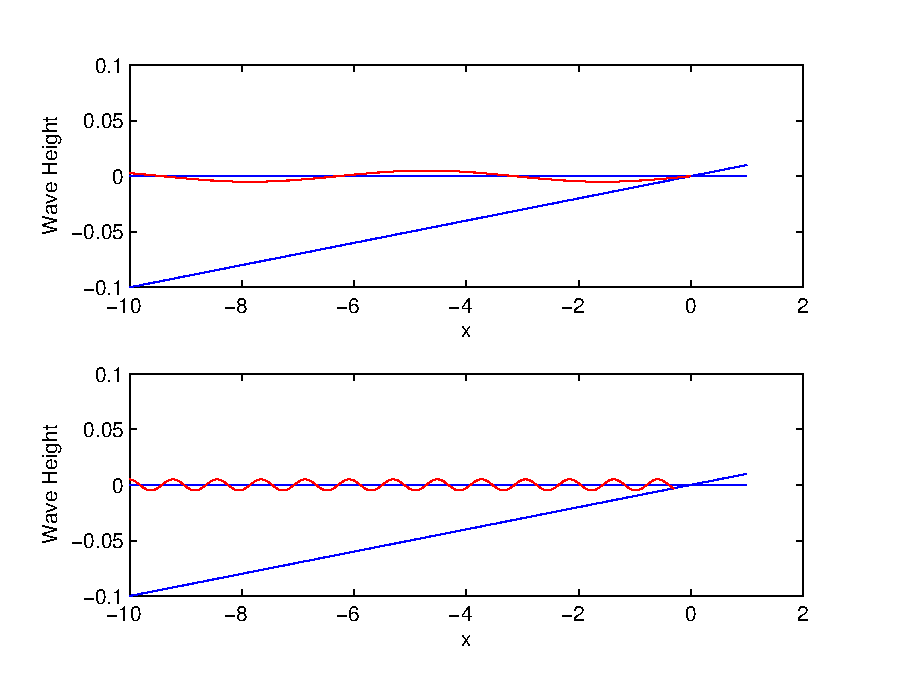
\includegraphics[width=.8\textwidth]{bay/wave_comp.eps}
	}
% 1.1.1  Typical causes of tsunami waves
	\slide[Causes of Tsunami Waves] {
	\begin{tabular}{|l|l|}\hline
		Rock Slides--Chehalis Lake&Earthquakes\\
			 \includegraphics[width=.4\textwidth]{causes/Landslide.jpg}%http://wikimapia.org/22797805/Chehalis-Lake-Rock-Slide
			&\includegraphics[width=.5\textwidth]{causes/Earrthquake.png}\\\hline%http://www.enchantedlearning.com/subjects/tsunami/\\\hline
			Asteroid Impact&Glacier Calving\\
			 ~ ~ \includegraphics[width=.3\textwidth]{causes/Asteroid.jpg}%http://mail.colonial.net/~hkaiter/asteroidbelt.html
			&\includegraphics[width=.5\textwidth]{causes/Calving.jpg}\\\hline
	\end{tabular}
	}


\slide[Purpose of Research]{
\bi	\item Faster numerical modeling of wave run-up
	\bi	\item Closed bays with a steep wall
		\item Carrier-Greenspan transformation generalized by Rybkin-Pelinovsky-Didenkulova.
		\item $<1$ min vs. 2 days computation time
	\ei
\ei
}
% 1.1.2  Include pictures/videos ? from trip and elsewhere
% 1.2  Purpose of our research
	\slide[Introduction to the Problem]{
		Mathematical modeling of tsunami run-up
		\bi	\item Numerous real-world applications
			\item Involves solving non-linear partial differential equations
		\ei
		Our REU program focused on
		\bi	\item Bays of U-Shaped bays of finite length.
			\item Spectral method for finding numerical series solutions.
		\ei
	}
	
	
	\slide [Introduction to the Bay Shapes]{
		In the field of Tsunami run-up research, there are several natural bay shapes to examine:
		\begin{itemize}
			\item The plane beach;
			\item Bays of parabolic cross-section;
		\end{itemize}
		There has been extensive study of the plane beach and bays of parabolic cross-section, but tsunami behavior in bays of general U-shaped bays of finite length has not been examined.
		
		In each case, we assume that the bottom profile is separable: \emph{i.e.}
		\[   z(x,y) = f(y) - h(x)  \]
		where $z(x,y)$ is the bottom profile, $f(y)$ is an arbitrary function and $h(x)$ is an arbitrary non-negative function.
	}

	\slide[The Plane Beach]{\includegraphics[width=\linewidth]{bay/planebeach.png}}

	\slide[The Plane Beach]{
		Characteristics of the plane beach:
		\begin{itemize}
			\item Constant slope;
			\item Uniform across y-axis;
			\item Can be simplified to 2 dimensions.
		\end{itemize}
		This is the problem examined in the famous 1958 paper of Carrier and Greenspan.
		They showed that in this case, explicit solutions to the shallow water wave equations were possible.
	}

	\slide[Bays of Parabolic Cross-section]{\includegraphics[width=\linewidth]{bay/parabolicbay.png}}

	\slide[Bays of Parabolic Cross-section]{
		Characteristics of bays of parabolic cross-section:
		Characteristics of bays of parabolic cross-section:
		\begin{itemize}
			\item Constant slope;
			\item Parabolic cross-section along y-axis;
			\item Behavior of waves in such a channel can still be simplified to 2 dimensions.
		\end{itemize}
		This more complicated problem was analyzed in a recent paper by Dr. Ira Didenkulova and Dr. Efim Pelinovsky,
			in which they showed that it was possible to reduce this problem to one that is analogous to the 2-dimensional case,
			and thus analytical solutions are possible for the infinite length case.
	}

	\slide[Bays of Trapezoidal Cross-section]{\includegraphics[width=\linewidth]{bay/trapezoidalbay.png}}

	\slide[Bays of Trapezoidal Cross-section]{
		Characteristics of bays of trapezoidal cross-section:
		\begin{itemize}
			\item Constant slope
			\item Cross-section is determined by a symmetrical trapezoid\\
			slope of the walls is $\beta$\\
			distance across the base is $2 y_0$
			\item Behavior of waves in such a bay is unknown. 
		\end{itemize}
		These bays where the focus of the 2012 REU.
	}

	\slide[Terminology]{
		\begin{itemize}
			\item $\eta(x,t)$ is the perturbation of water level at time $t$, distance $x$ from shore.
			\item $H(x,t)$ is the total water depth. Note: $H(x,t) = h(x) + \eta(x,t)$.
			\item $S(H)$ is the cross-sectional area of the bay. Note
				\[ S(H) = \int_0^{H(x,t)} f(y) \delta y \]
			\item $u(x,t)$ is the average water velocity on a cross-section perpendicular to the cross-section.
			\item We only consider $h(x) = -\alpha x$, where $\alpha$ is a non-negative constant. Since $x$ is typically negative in our domain, $h$ will usually be non-negative, and $H$ must always be non-negative.
		\end{itemize}
	}
